\documentclass[]{article}
\usepackage{lmodern}
\usepackage{amssymb,amsmath}
\usepackage{ifxetex,ifluatex}
\usepackage{fixltx2e} % provides \textsubscript
\ifnum 0\ifxetex 1\fi\ifluatex 1\fi=0 % if pdftex
  \usepackage[T1]{fontenc}
  \usepackage[utf8]{inputenc}
\else % if luatex or xelatex
  \ifxetex
    \usepackage{mathspec}
    \usepackage{xltxtra,xunicode}
  \else
    \usepackage{fontspec}
  \fi
  \defaultfontfeatures{Mapping=tex-text,Scale=MatchLowercase}
  \newcommand{\euro}{€}
\fi
% use upquote if available, for straight quotes in verbatim environments
\IfFileExists{upquote.sty}{\usepackage{upquote}}{}
% use microtype if available
\IfFileExists{microtype.sty}{%
\usepackage{microtype}
\UseMicrotypeSet[protrusion]{basicmath} % disable protrusion for tt fonts
}{}
\usepackage[margin=1in]{geometry}
\usepackage{graphicx}
\makeatletter
\def\maxwidth{\ifdim\Gin@nat@width>\linewidth\linewidth\else\Gin@nat@width\fi}
\def\maxheight{\ifdim\Gin@nat@height>\textheight\textheight\else\Gin@nat@height\fi}
\makeatother
% Scale images if necessary, so that they will not overflow the page
% margins by default, and it is still possible to overwrite the defaults
% using explicit options in \includegraphics[width, height, ...]{}
\setkeys{Gin}{width=\maxwidth,height=\maxheight,keepaspectratio}
\ifxetex
  \usepackage[setpagesize=false, % page size defined by xetex
              unicode=false, % unicode breaks when used with xetex
              xetex]{hyperref}
\else
  \usepackage[unicode=true]{hyperref}
\fi
\hypersetup{breaklinks=true,
            bookmarks=true,
            pdfauthor={Ismay Pérez Sánchez},
            pdftitle={Study of predictors of miles per gallon (MPG)},
            colorlinks=true,
            citecolor=blue,
            urlcolor=blue,
            linkcolor=magenta,
            pdfborder={0 0 0}}
\urlstyle{same}  % don't use monospace font for urls
\setlength{\parindent}{0pt}
\setlength{\parskip}{6pt plus 2pt minus 1pt}
\setlength{\emergencystretch}{3em}  % prevent overfull lines
\setcounter{secnumdepth}{0}

%%% Use protect on footnotes to avoid problems with footnotes in titles
\let\rmarkdownfootnote\footnote%
\def\footnote{\protect\rmarkdownfootnote}

%%% Change title format to be more compact
\usepackage{titling}
\setlength{\droptitle}{-2em}
  \title{Study of predictors of miles per gallon (MPG)}
  \pretitle{\vspace{\droptitle}\centering\huge}
  \posttitle{\par}
  \author{Ismay Pérez Sánchez}
  \preauthor{\centering\large\emph}
  \postauthor{\par}
  \predate{\centering\large\emph}
  \postdate{\par}
  \date{23/05/2015}




\begin{document}

\maketitle


\subsection{Executive summary}\label{executive-summary}

This study has the purpose of determine the relationship between a set
of variables and miles per gallon (MPG). The data used are the
\texttt{mtcar} dataset available as a package of R, collected on
previous studies some decades ago.\\The tasks that will be performed
aims to solve the question of which kind of transmission is better for
MPG and how different are they. The results indicate that Manual
transmission is better than Automatic in about 3 mpg.\\For a more
detailed document to reproduce this go to
\url{https://github.com/mooc-only/regression_models}

\subsection{Exploratory data analyses}\label{exploratory-data-analyses}

First, we will check how each kind of transmission affect independently
to MPG. The \texttt{figure 1} (Appendix) constructed as a boxplot to
show the distribution of MPG for each level of \texttt{am} variable
(representing transmission), give us at first glace a very clear
tendency of manual transmission to outperform automatic one. In
\texttt{figure 2} are shown multiples plots in which can be selected
\textbf{cyl}, \textbf{displ}, \textbf{hp}, \textbf{wt}, \textbf{vs},
\textbf{am} as the variables that visibly are correlated with MPG.

\subsection{Statistical Inference for corroboration of visual comparison
of transmission
type}\label{statistical-inference-for-corroboration-of-visual-comparison-of-transmission-type}

Assuming normality in the MPG data by each kind of transmission we can
make a T-test
(\texttt{t.test(mpg \textasciitilde{} am, data=mtcars, alternative="greater", paired=F)}
after leveling the manual type) with the following hypothesis:

$H_{0}$: MPG with manual transmission is less than with
automatic.\\$H_{1}$: MPG with manual transmission is greater than with
automatic.

Obtaining a p-value of 0.00069 with which we reject the null hypothesis
and accept that manual transmission is better producing more miles per
gallon.

\subsection{Regression model}\label{regression-model}

In order to quantify how different is the MPG between the transmissions
we will create various models that fit as better as possible the
behavior of the outcome, compare them with ANOVA criterion and perform
some diagnostics on residuals.

The first candidate will be computed with the stepwise procedure
(\texttt{step} function in R) using default parameter for direction
`both' (i.e: forward selection and backward elimination). The resultant
model is constructed as mpg \textasciitilde{} wt + qsec + am.

For the other models, will be computed the correlations of all
predictors with the outcome (MPG). Then, turn positive the negatives
(because the magnitude is what it is important, the sign only shows the
direction), sort them and calculate the differences between consecutive
predictors. All the differences are under \texttt{0.1} (\texttt{10\%}
increase of correlation between closest predictors) what results in
values somewhat spread between \texttt{0.005} and \texttt{0.09} (an
additional analysis could be appropriate, but the space limits my will).
The last values -more correlated predictors- concentrate the lowest
differences, what makes the upper half of the list ( drat + hp + disp +
cyl + wt) a clear separations to create an initial set for another
model, but \textbf{am} is not between them, so it does not make sense
for our purpose. Instead, we will create another models with all
variables more correlated than \textbf{am}, including it, and a refined
model with \texttt{step} function.

The new models are (mpg \textasciitilde{} am + vs + drat + hp + disp +
cyl + wt) and the refined (mpg \textasciitilde{} hp + cyl + wt), this
lack of interest because \textbf{am} are not in it. ANOVA test shows
that reject $H_{0}$ for the 1st pair of models, thus, \textbf{wt} and
\textbf{qsec} indeed improve the accuracy of the model over the basic
(\texttt{mpg \textasciitilde{} am}). But fail to reject $H_{0}$ in the
second, therefore, none of the models has significant difference over
the other.

\begin{verbatim}
## Analysis of Variance Table
## 
## Model 1: mpg ~ am
## Model 2: mpg ~ wt + qsec + am
## Model 3: mpg ~ am + vs + drat + hp + disp + cyl + wt
##   Res.Df    RSS Df Sum of Sq       F    Pr(>F)    
## 1     30 720.90                                   
## 2     28 169.29  2    551.61 41.7217 1.543e-08 ***
## 3     24 158.65  4     10.63  0.4021    0.8052    
## ---
## Signif. codes:  0 '***' 0.001 '**' 0.01 '*' 0.05 '.' 0.1 ' ' 1
\end{verbatim}

But the following analysis will be done with the model resultant from
the initial stepwise algorithm because it has the higher sample
correlation squared, meaning that explain better the variability in the
sample (check that it is included the model discarded for not having
\textbf{am} only to show that it cover less too).

\begin{verbatim}
##                                        formula RSquared
## 1                         mpg ~ wt + qsec + am  0.83356
## 2 mpg ~  am + vs + drat + hp + disp + cyl + wt  0.81801
## 3                          mpg ~ hp + cyl + wt  0.82634
\end{verbatim}

\subsection{Residual plots and some
diagnostics}\label{residual-plots-and-some-diagnostics}

In the \texttt{figure 3} there are many plots with the redisual
analysis. Residual vs Fitted shows independence, Normal Q-Q indicate
that the residuals are normally distributed and Scale-Location that
variance is constant. There are some points (3 in each plot) that are
interesting to check. The 3 points with most leverage are found with the
\texttt{hatvalues()} function.

\begin{verbatim}
##   Chrysler Imperial Lincoln Continental            Merc 230 
##           0.2296338           0.2642151           0.2970422
\end{verbatim}

And those with most influence using \texttt{dfbetas()}.

\begin{verbatim}
##     Toyota Corona          Fiat 128 Chrysler Imperial 
##         0.4050410         0.4765680         0.5626418
\end{verbatim}

Coincidentally are mostly the same points saw at the plots.

\section{Regression Model
interpretation}\label{regression-model-interpretation}

Given the coefficients of the selected model:

\begin{verbatim}
## (Intercept)          wt        qsec    amManual 
##    9.617781   -3.916504    1.225886    2.935837
\end{verbatim}

Manual transmission improve Automatic transmission in almost 3 miles per
gallon.\\The miles per gallon will increase by 1.2 for every qsec (1/4
mile time).\\For every ton increase in weight the cars will decrease
approximately 4 miles per gallon.

\section{Appendix}\label{appendix}

Figure 1

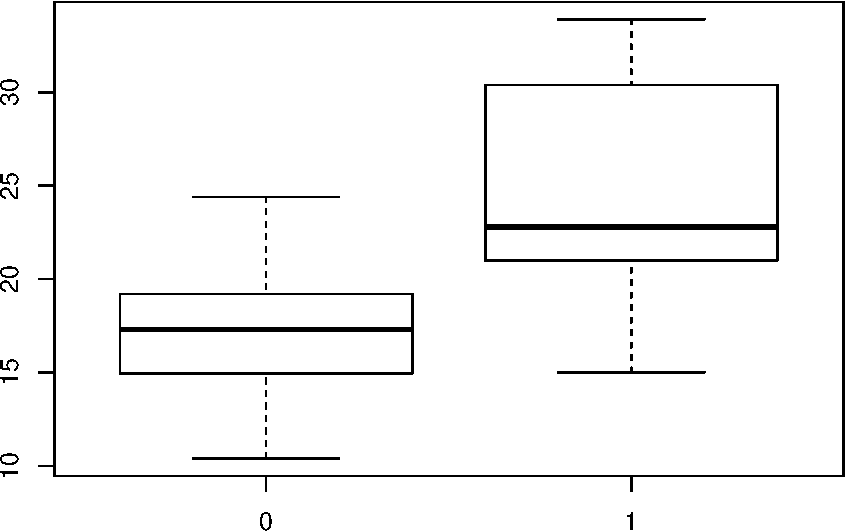
\includegraphics{assigment_files/figure-latex/unnamed-chunk-11-1.pdf}

Figure 2

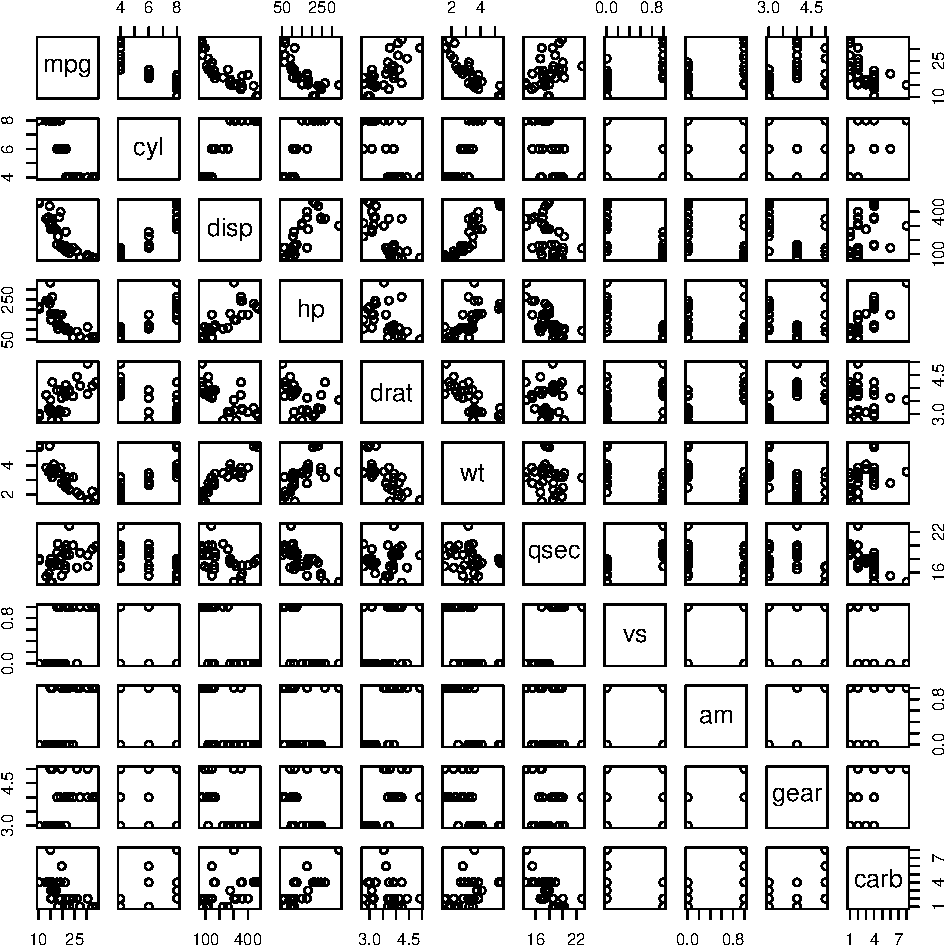
\includegraphics{assigment_files/figure-latex/unnamed-chunk-12-1.pdf}

Figure 3

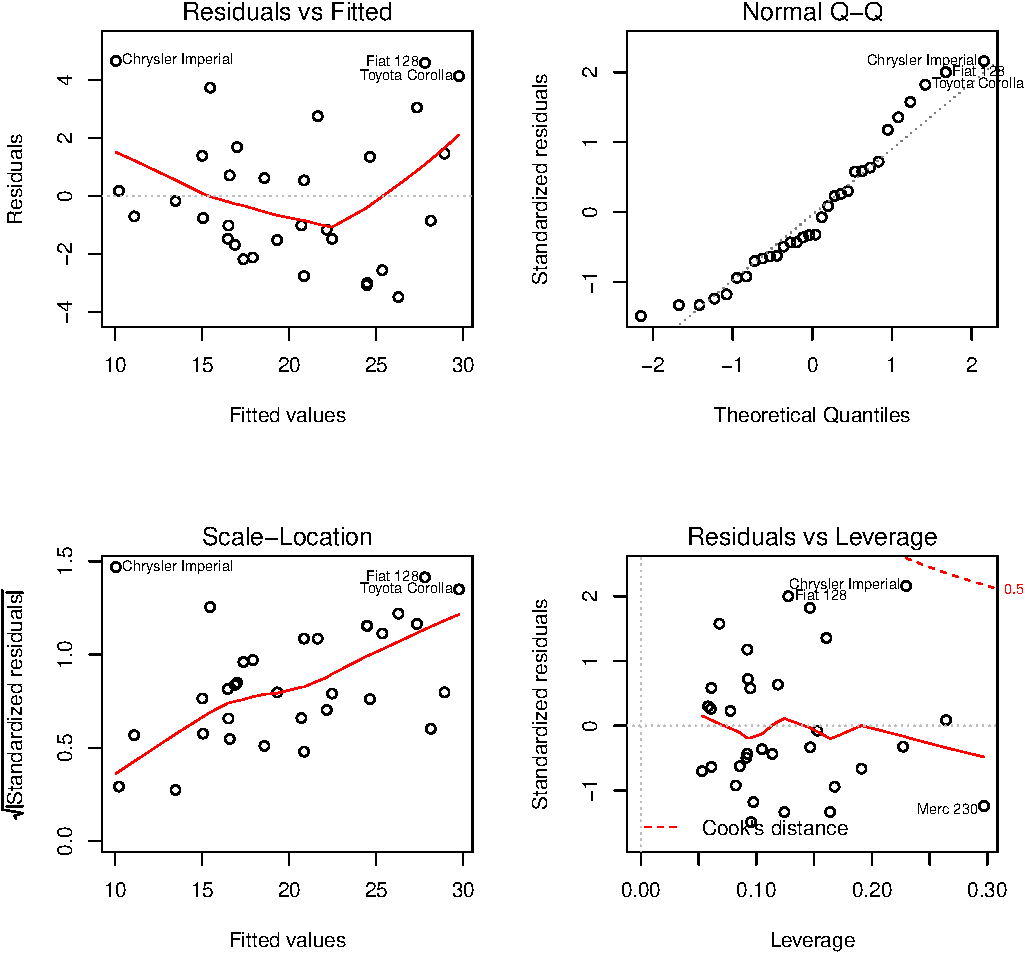
\includegraphics{assigment_files/figure-latex/unnamed-chunk-13-1.pdf}

\end{document}
